
\documentclass[runningheads,a4paper]{llncs}

\usepackage{amssymb}
\setcounter{tocdepth}{3}
\usepackage{graphicx}

\usepackage{url}
\usepackage{listings}
\usepackage[a4paper, margin=1in]{geometry}

\begin{document}

\mainmatter  % start of an individual contribution

% first the title is needed
\title{Clustering techniques for Customer Segmentation in Credit Card Usage Data}

% a short form should be given in case it is too long for the running head
\titlerunning{Clustering techniques}


\author{Anushka Darade \and Payal Nagaonkar \and Ritesh Choudhary }

\authorrunning{Anushka Darade, Payal Nagaonkar \& Ritesh Choudhary}
% (feature abused for this document to repeat the title also on left hand pages)

% the affiliations are given next
\institute{Northeastern University}


\maketitle

\begin{abstract}
Customer segmentation is a critical task for businesses aiming to optimize marketing strategies and offer personalized services. In this study, we analyze the credit card behavior of 9,000 active customers using multiple clustering techniques, including \textit{KMeans}, \textit{Hierarchical Clustering}, \textit{DBSCAN}, and \textit{Gaussian Mixture Models (GMM)}. Each clustering algorithm is evaluated based on key metrics such as the \textit{Silhouette Score}, \textit{Calinski-Harabasz Index}, and \textit{Davies-Bouldin Index} to identify the most effective method for customer segmentation. \textit{Hierarchical Clustering} and \textit{KMeans}, particularly after dimensionality reduction through PCA, performed best, with \textit{Hierarchical Clustering} achieving a \textit{Silhouette Score} of 0.8543, indicating well-defined clusters. We further identify distinct customer groups, such as high spenders, installment-focused customers, and cash advance-heavy users, providing valuable insights into customer behavior. The results demonstrate that effective segmentation can enable businesses to tailor their offerings to specific customer needs, thereby improving engagement and financial outcomes. Additionally, we propose future improvements, including the use of advanced clustering techniques and incorporating external data for richer analysis.

\keywords{Customer segmentation, clustering techniques, KMeans, hierarchical clustering, DBSCAN, spectral clustering, Gaussian Mixture Models (GMM).}
\end{abstract}



\section{Introduction}

In today's data-driven economy, businesses continuously strive to understand customer behavior to tailor their marketing strategies, improve customer experience, and drive profitability. One of the most powerful tools for achieving this understanding is customer segmentation—the process of dividing a broad consumer base into distinct groups, each characterized by unique patterns of behavior, preferences, and needs. By accurately segmenting customers, businesses can design more personalized marketing campaigns, enhance product offerings, and improve customer retention rates. Among the various methods for customer segmentation, clustering techniques have emerged as a key approach, especially in industries with large volumes of transactional data, such as credit card usage.

Credit card usage data provides rich insights into customer behavior, offering a window into spending patterns, payment habits, and financial preferences. However, analyzing and extracting actionable insights from this data is a complex task, given the variability in individual behavior and the large volume of transactions. Traditional marketing methods may not effectively capture these nuances, leading to generalized strategies that fail to resonate with specific customer groups. This is where clustering techniques come into play, enabling companies to group customers based on their behavior and allowing for more targeted marketing strategies.

Clustering, a type of unsupervised machine learning, aims to automatically group customers into segments that exhibit similar behaviors or characteristics. These techniques help reveal hidden patterns in the data, making it easier for businesses to understand customer needs at a granular level. By leveraging clustering algorithms, companies can identify high-value customers, detect emerging trends, and refine their customer engagement strategies. Furthermore, segmentation based on clustering can assist in optimizing resource allocation, as businesses can focus their efforts on the most profitable or high-potential customer segments.

This paper explores various clustering techniques applied to customer segmentation in credit card usage data, discussing their effectiveness in uncovering behavioral patterns and their impact on marketing strategies. We will examine common algorithms such as K-means, hierarchical clustering, and DBSCAN, highlighting their strengths, limitations, and applicability in different business scenarios. Additionally, we will assess the relevance of these methods in generating actionable insights for marketing and customer relationship management.

\section{Literature Review}

A substantial body of research has been dedicated to customer segmentation using clustering techniques, particularly in industries with high volumes of transactional data. The application of clustering in financial services, such as credit card usage, has gained significant attention due to the growing availability of detailed transaction-level data and advances in machine learning.

Customer segmentation using clustering algorithms has been extensively studied across various domains, with researchers emphasizing its importance in providing actionable insights for business strategy. Several studies have highlighted the value of clustering in identifying key customer segments that are not easily identifiable through traditional methods. For instance, Xu and Tian (2015) explored the use of K-Means and DBSCAN in customer segmentation, concluding that while K-Means is effective for homogeneous clusters, DBSCAN excels in discovering irregular patterns in spending behavior, making it ideal for financial datasets.

Many studies have explored the use of K-Means clustering for customer segmentation. Jain and Dubes (2008) highlighted the simplicity and effectiveness of K-Means in customer behavior segmentation, particularly in structured data such as transactional histories. However, they also pointed out the limitations of K-Means in handling outliers and irregular cluster shapes, which are common in real-world data.

Hierarchical clustering has been widely applied in customer segmentation due to its flexibility in creating a tree-like structure of customer groups. Tan et al. (2016) emphasized that hierarchical clustering is particularly useful when the data exhibits a nested structure, such as tiered customer loyalty programs or membership levels. However, due to its computational complexity, hierarchical clustering is less suited for large-scale data, limiting its application in credit card usage datasets with millions of transactions.

Studies have also highlighted DBSCAN's ability to detect clusters in financial datasets, particularly for customers with irregular spending patterns or atypical behaviors. A study by Ester et al. (1996), who introduced DBSCAN, demonstrated its advantages in discovering clusters of varying densities and its robustness to noise. In the context of credit card usage, where customer behavior can vary widely, DBSCAN has been shown to outperform traditional methods in uncovering hidden patterns (Ngai et al., 2009).

Ngai et al. (2009) and Saraswat et al. (2013) explored various clustering techniques in the financial sector, particularly focusing on credit card data. Their research indicated that behavioral segmentation using clustering techniques can lead to more precise targeting of high-value customers, fraud detection, and improved credit risk assessment. They demonstrated that clustering could reveal spending patterns, such as frequent small transactions versus large one-off purchases, which are indicative of different customer segments.

In conclusion, the literature underscores the significance of clustering techniques in customer segmentation, particularly in industries dealing with vast amounts of behavioral data. As the financial sector becomes increasingly reliant on data-driven decision-making, clustering continues to offer valuable insights into customer behavior, enabling businesses to craft more effective marketing strategies and improve operational efficiencies.


\section{Theory \& Background}

Customer segmentation is a vital process in marketing and business analytics, where the goal is to divide a heterogeneous customer base into homogeneous groups based on common attributes, behaviors, or preferences. Segmentation enables businesses to tailor marketing strategies, optimize resources, and improve customer experience by addressing the distinct needs of each segment. Traditionally, segmentation was based on demographic or psychographic factors. However, with the advent of big data, businesses have shifted towards behavior-based segmentation, particularly in industries with extensive transactional data, such as credit card usage.

Clustering is a type of unsupervised machine learning, where the primary aim is to group data points that are similar to one another while maximizing the differences between clusters. It differs from supervised learning, where a labeled dataset is used to train models. Instead, clustering works without predefined labels, relying on algorithms to identify inherent patterns within the data. For customer segmentation, clustering helps identify distinct groups of customers with similar spending behaviors, usage patterns, or risk profiles, enabling more targeted marketing approaches.

Clustering algorithms are widely used in customer segmentation. The most common techniques used are classified based on the following parameters:

\textbf{\emph{1. Centroid-based:}} A popular centroid-based method that partitions customers into K clusters, called K-Means Clustering, is used by minimizing the distance between individual data points and their respective cluster centroids.

\textbf{\emph{2. Hierarchy-based:}} This approach builds a hierarchy of clusters, called Hierarchical Clustering, either by agglomerative (bottom-up) or divisive (top-down) techniques. It is well-suited for identifying a nested structure in the data but is computationally expensive.

\textbf{\emph{3. Density-based:}} A density-based algorithm, called Density-Based Spatial Clustering of Applications with Noise (DBSCAN), that forms clusters based on the density of points in a region. Unlike K-means, DBSCAN can detect arbitrarily shaped clusters and handle noise in the data.

Each of these techniques comes with its strengths and limitations. For example, K-Means is computationally efficient but struggles with non-spherical cluster shapes and sensitivity to outliers. In contrast, DBSCAN is better for discovering clusters of varying shapes and is robust to noise but may struggle with high-dimensional data.

In the context of credit card usage data, clustering algorithms help segment customers based on behavioral factors such as spending habits, payment patterns, and credit utilization. These insights are invaluable for developing targeted marketing strategies, such as personalized offers or risk management policies.

\subsection{Problem Statement}

In the highly competitive financial services sector, understanding customer behavior is crucial for developing effective marketing strategies and improving customer retention. One of the most significant challenges faced by credit card companies is the effective segmentation of their customer base. Traditional segmentation methods often fail to capture the complexity and nuances of customer behavior, leading to less targeted marketing efforts and missed opportunities for enhancing customer satisfaction.

The objective of this research is to apply clustering techniques to credit card usage data to identify distinct customer segments based on their behavioral patterns. The dataset comprises 18 behavioral variables that provide insights into customers' financial behaviors, including their purchasing habits, payment behaviors, and account balances. By utilizing clustering algorithms, we aim to generate meaningful groups that represent different segments of customers, each with unique characteristics and needs. \\

\textbf{Input:} The dataset contains 18 behavioral variables that reflect various aspects of customer behavior. The variables include:
\\
\textbf{1. CUST\_ID:} Identification of Credit Card holder (Categorical) \\
\textbf{2. BALANCE:} Balance amount left in their account to make purchases (Numerical) \\
\textbf{3. BALANCE\_FREQUENCY:} How frequently the balance is updated, scored between 0 and 1 (Numerical) \\
\textbf{4. PURCHASES:} Amount of purchases made from the account (Numerical) \\
\textbf{5. ONEOFF\_PURCHASES:} Maximum purchase amount done in one-go (Numerical) \\
\textbf{6. INSTALLMENTS\_PURCHASES:} Amount of purchase done in installments (Numerical) \\
\textbf{7. CASH\_ADVANCE:} Cash in advance given by the user (Numerical) \\
\textbf{8. PURCHASES\_FREQUENCY:} How frequently purchases are being made, scored between 0 and 1 (Numerical) \\
\textbf{9. ONEOFFPURCHASESFREQUENCY:} Frequency of one-off purchases, scored between 0 and 1 (Numerical) \\
\textbf{10. PURCHASESINSTALLMENTSFREQUENCY:} Frequency of installment purchases, scored between 0 and 1 (Numerical) \\
\textbf{11. CASHADVANCEFREQUENCY:} Frequency of cash advances (Numerical) \\
\textbf{12. CASHADVANCETRX:} Number of transactions made with cash advances (Numerical) \\
\textbf{13. PURCHASES\_TRX:} Number of purchase transactions made (Numerical) \\
\textbf{14. CREDIT\_LIMIT:} Credit limit for the user (Numerical) \\
\textbf{15. PAYMENTS:} Amount of payment done by the user (Numerical) \\
\textbf{16. MINIMUM\_PAYMENTS:} Minimum amount of payments made by the user (Numerical) \\
\textbf{17. PRCFULLPAYMENT:} Percentage of full payment made by the user (Numerical) \\
\textbf{18. TENURE:} Tenure of credit card service for the user (Numerical) \\
\\
\textbf{Output:} The output will be a set of clusters that categorize customers into distinct segments based on their behavioral characteristics. Each cluster will represent a group of customers with similar spending habits, payment behaviors, and financial management patterns. For example, we might identify clusters such as: 
\\
\textbf{Cluster A:} High spenders with frequent one-off purchases and a high credit limit. \\
\textbf{Cluster B:} Moderate spenders who predominantly use installments and have low cash advance transactions. \\
\textbf{Cluster C:} Low activity users with infrequent purchases and low balances. \\

By analyzing these clusters, credit card companies can tailor marketing strategies, improve customer engagement, and enhance service offerings to meet the specific needs of each customer segment.

\section{Research Methodology}

The following section describes the clustering techniques applied to segment credit card holders based on their behavioral attributes. Each algorithm was chosen based on its strengths in handling specific data characteristics, and the mathematical foundations, implementation steps, and hyperparameter tuning strategies are outlined in detail.

\subsection{KMeans Clustering}

KMeans clustering was selected as the baseline algorithm due to its simplicity and computational efficiency in partitioning data into compact, spherical clusters. The objective of KMeans is to minimize the within-cluster sum of squares (WCSS), formally expressed as:

\begin{equation}
J = \sum_{i=1}^{k} \sum_{x_j \in C_i} \| x_j - \mu_i \|^2
\end{equation}

where \( C_i \) is the cluster \( i \), \( \mu_i \) is the centroid of cluster \( i \), and \( \| x_j - \mu_i \|^2 \) represents the squared Euclidean distance between point \( x_j \) and the centroid. The number of clusters \( k \) was determined using the Elbow Method, which plots the WCSS for varying values of \( k \). The point where the reduction in WCSS becomes marginal (the “elbow”) was chosen as the optimal number of clusters, yielding \( k = 5 \) for this dataset. 

KMeans iteratively assigns points to the nearest centroid, updates the centroids as the mean of the points in each cluster, and repeats until convergence. This approach was suitable given the relatively large dataset and the expectation of well-separated customer segments based on behavioral attributes. However, KMeans assumes spherical clusters and is sensitive to outliers, which were addressed by standardizing the data prior to clustering. The algorithm was initialized multiple times with different random centroid placements to avoid local minima.

\begin{itemize}
    \item Randomly initialize \( k \) centroids \( \mu_1, \mu_2, ..., \mu_k \in \mathbb{R}^n \).
    \item Repeat until convergence:
    \begin{itemize}
        \item Assign each point \( x_j \) to the nearest centroid:
        \[
        c^{(i)} = \arg\min_{j} \| x_j - \mu_j \|^2
        \]
        \item Update each centroid \( \mu_j \) as the mean of the points in cluster \( j \):
        \[
        \mu_j = \frac{1}{|C_j|} \sum_{i=1}^{m} 1(c^{(i)} = j) x^{(i)}
        \]
    \end{itemize}
    \item Return final cluster assignments and centroids.
\end{itemize}

\subsection{Hierarchical Clustering}

Hierarchical clustering was implemented to explore the nested structure of the data without predefining the number of clusters. The agglomerative method was chosen, where each point starts as its own cluster, and clusters are successively merged based on their similarity. We used Ward’s linkage, which minimizes the total within-cluster variance. The merging criterion is mathematically represented as:

\begin{equation}
d(A, B) = \frac{n_A n_B}{n_A + n_B} \| \mu_A - \mu_B \|^2
\end{equation}

where \( n_A \) and \( n_B \) are the sizes of clusters \( A \) and \( B \), and \( \mu_A \), \( \mu_B \) represent their centroids. This method is particularly effective for forming compact, well-separated clusters. The dendrogram generated from hierarchical clustering provided a visual representation of the cluster hierarchy, and the optimal number of clusters was selected by cutting the tree at the point with the largest vertical distance between merges.

This approach was ideal for detecting subclusters within larger groups, providing insight into the hierarchical structure of customer segments. However, hierarchical clustering is computationally expensive with a time complexity of \( O(n^3) \), making it less scalable for very large datasets.

\begin{verbatim}
# Hierarchical Clustering algorithm
# Input: Data X
# Output: Dendrogram and cluster assignments

1. Start with each point as a single cluster.
2. Compute pairwise distances between clusters.
3. Repeat until only one cluster remains:
   a. Merge the two closest clusters based on Ward’s linkage.
   b. Recompute the distance matrix.
4. Cut the dendrogram to obtain the desired number of clusters.
\end{verbatim}

\subsection{DBSCAN}

DBSCAN was chosen for its ability to discover clusters of arbitrary shapes and handle noise, which is critical given the potential for outliers in customer behavior. Unlike KMeans and hierarchical clustering, DBSCAN does not require specifying the number of clusters beforehand. Instead, it identifies core points—those with at least a specified number of neighbors within a certain radius—and groups points that are density-reachable. Points that are not reachable from any core point are classified as noise (outliers).

The key hyperparameters for DBSCAN are \( \varepsilon \) (the neighborhood radius) and `minsamples` (the minimum number of points required to form a dense region). These were tuned using a k-distance plot, where \( \varepsilon \) was selected at the point where the distance between the \( k \)-th nearest neighbors shows a sharp increase. 

\begin{itemize}
    \item For each point \( p \) in the dataset \( X \):
    \begin{itemize}
        \item If \( p \) has more than `min\_samples` neighbors within a distance \( \varepsilon \), mark it as a core point.
        \item Expand the cluster by recursively including all density-reachable points.
    \end{itemize}
    \item Mark points that are not reachable as noise.
\end{itemize}

This method was effective in isolating customers with atypical behaviors, which were treated as outliers.

\subsection{Spectral Clustering}

Spectral Clustering was employed to address potential non-linear separability in the data. Spectral clustering constructs a graph where nodes represent data points, and edges represent the similarity between points. A similarity matrix \( W \) was computed using the Gaussian kernel:

\begin{equation}
W_{ij} = \exp\left(-\frac{\| x_i - x_j \|^2}{2\sigma^2}\right)
\end{equation}

where \( \sigma \) controls the width of the Gaussian kernel. The Laplacian matrix \( L \) was then computed as:

\begin{equation}
L = D - W
\end{equation}

where \( D \) is the degree matrix. The first \( k \) eigenvectors of \( L \) were computed, and KMeans was applied to cluster the data in this reduced eigenvector space. This approach is particularly effective in detecting clusters that are non-linearly separable in the original space. Spectral clustering was applied after constructing the similarity matrix from the credit card behavioral features, providing a deeper understanding of the intrinsic structure of customer groups.

\begin{verbatim}
# Spectral Clustering algorithm
# Input: Data X, number of clusters k
# Output: Cluster assignments

1. Construct similarity matrix W using Gaussian kernel.
2. Compute Laplacian matrix L = D - W.
3. Find the first k eigenvectors of L.
4. Apply KMeans on the eigenvectors.
5. Return cluster assignments.
\end{verbatim}

\subsection{Gaussian Mixture Models (GMM)}

Gaussian Mixture Models (GMM) were used to model the data as a mixture of Gaussian distributions, allowing for soft clustering where each point is assigned a probability of belonging to each cluster. This was useful in scenarios where customers may exhibit overlapping behaviors (e.g., high spenders who also make frequent installment purchases). The probability density function of GMM is given by:

\begin{equation}
p(x) = \sum_{i=1}^{k} \pi_i \mathcal{N}(x \mid \mu_i, \Sigma_i)
\end{equation}

where \( \pi_i \) is the mixing coefficient, and \( \mathcal{N}(x \mid \mu_i, \Sigma_i) \) is the multivariate Gaussian distribution for cluster \( i \) with mean \( \mu_i \) and covariance \( \Sigma_i \). 

The Expectation-Maximization (EM) algorithm was used to estimate the parameters. The E-step computes the posterior probabilities of each point belonging to each Gaussian component, and the M-step updates the parameters to maximize the log-likelihood. The GMM algorithm was particularly useful in capturing customer behaviors that overlap across clusters, providing a more nuanced segmentation than hard clustering methods like KMeans. The GMM algorithm is outlined as follows:

\begin{itemize}
    \item Initialize parameters (means, covariances, mixing coefficients).
    \item Repeat until convergence:
    \begin{itemize}
        \item E-step: Compute posterior probabilities of each point belonging to each Gaussian component.
        \item M-step: Update parameters (means, covariances, mixing coefficients) to maximize the log-likelihood.
    \end{itemize}
    \item Assign points based on maximum posterior probability.
\end{itemize}

\section{Experimental Setup}

This study employs a systematic approach to segment credit card customers based on their behavioral patterns using five clustering techniques: KMeans, Hierarchical Clustering, DBSCAN, Spectral Clustering, and Gaussian Mixture Models (GMM). The process involves several key steps, including data preprocessing, application of clustering algorithms, and evaluation of results.

\subsection{Data Preprocessing}

The dataset comprises 9,000 credit card holders, each characterized by 18 behavioral variables, such as \textit{BALANCE}, \textit{PURCHASES}, and \textit{CREDIT LIMIT}. Before applying the clustering algorithms, the dataset was preprocessed to ensure consistency and improve the performance of the algorithms.

Initially, missing values were handled by imputing the median values for the \textit{MINIMUM PAYMENTS} and \textit{CREDIT LIMIT} variables, where significant gaps were observed. This method was chosen to minimize the influence of outliers and to retain as much data as possible for analysis.

Since the dataset includes variables with varying scales (e.g., \textit{BALANCE} values in thousands compared to \textit{BALANCE FREQUENCY}, which ranges from 0 to 1), all features were standardized using z-score normalization. This step was necessary to ensure that no single variable disproportionately influenced the clustering outcome, particularly in distance-based algorithms like KMeans and GMM.

To address the high dimensionality of the data, which can distort clustering results, Principal Component Analysis (PCA) was applied. PCA helped reduce the feature space while retaining 95\% of the dataset's variance, thereby improving both algorithm performance and interpretability of the clusters.

\subsection{Application of Clustering Techniques}

Five clustering algorithms were applied to the preprocessed dataset, each with a unique approach to identifying customer segments.

\textbf{KMeans Clustering} was used as a baseline algorithm, given its efficiency in partitioning data into distinct clusters by minimizing within-cluster variance. The optimal number of clusters was determined using the Elbow Method, where the sum of squared distances between points and their assigned centroids was plotted against varying values of $k$. The elbow point, where the rate of decrease in distance begins to flatten, was selected as the optimal number of clusters. Once the optimal $k$ was identified, KMeans was applied, iterating until the centroids stabilized.

\textbf{Hierarchical Clustering} was also employed, specifically using the agglomerative approach. This method does not require pre-specification of the number of clusters and instead builds a dendrogram that represents the nested structure of the clusters. Ward’s linkage criterion was used, which minimizes the total within-cluster variance at each step of the hierarchical merging process. The dendrogram was then analyzed to determine the most appropriate level of clustering based on the largest vertical distance between merges.

\textbf{DBSCAN (Density-Based Spatial Clustering of Applications with Noise)} was chosen for its ability to detect clusters of arbitrary shape and to identify outliers as noise. This is particularly important in behavioral datasets where customer patterns may not conform to spherical clusters. The parameters \textit{eps} (the neighborhood radius) and \textit{min\_samples} (the minimum number of points required to form a cluster) were tuned using a k-distance plot to optimize the density-based clustering.

\textbf{Spectral Clustering} was employed to address potential non-linear relationships between features, which may not be captured by traditional distance-based clustering methods. Spectral Clustering transforms the data into a similarity graph and uses the eigenvalues of the Laplacian matrix to reduce the dimensionality before applying clustering in this lower-dimensional space. This method is effective in separating clusters when the data exhibits non-convex structures.

Finally, \textbf{Gaussian Mixture Models (GMM)} were applied to the dataset to enable soft clustering, where each data point is assigned a probability of belonging to multiple clusters. GMM assumes that the data is generated from a mixture of Gaussian distributions, providing a flexible clustering approach. The Bayesian Information Criterion (BIC) was used to select the optimal number of components (clusters), balancing model fit and complexity.

\subsection{Addressing Constraints and Challenges}

Throughout the analysis, several challenges were addressed to ensure meaningful and interpretable customer segments. The high dimensionality of the dataset was mitigated through PCA, which reduced the feature space while preserving the variance needed for effective clustering. Standardization of features ensured that variables with large magnitudes, such as \textit{BALANCE} and \textit{CREDIT LIMIT}, did not overshadow the smaller-scale features like \textit{BALANCE FREQUENCY}.

The detection of outliers, which could distort the clustering results, was achieved through the application of DBSCAN, a density-based algorithm that effectively isolates noise. The optimal number of clusters for algorithms such as KMeans and GMM, which require pre-specification, was determined through methods like the Elbow Method and BIC. These techniques ensured that the clusters formed were both meaningful and interpretable, balancing intra-cluster cohesion and inter-cluster separation.

\subsection{Evaluation Metrics}

To evaluate the performance of the clustering algorithms, several validation metrics were employed. The \textbf{Silhouette Coefficient} was used to measure how similar each point is to its assigned cluster compared to other clusters, providing insight into the cohesion and separation of the clusters. Additionally, the \textbf{Davies-Bouldin Index} was applied to assess the ratio of within-cluster scatter to between-cluster separation, with lower values indicating better-defined clusters.

Visual inspection of the clusters was performed using scatter plots and heatmaps, which helped validate the cluster assignments by analyzing key behavioral features across different customer segments. These visualizations allowed for better interpretation of the results, especially in understanding how certain variables, such as \textit{PURCHASES\_FREQUENCY} and \textit{PAYMENTS}, varied across different clusters.

\section{Observations \& Results}

\subsection{KMeans Clustering}

The KMeans algorithm was applied to the dataset without any transformation. The Elbow Method was used to determine the optimal number of clusters (see Figure \ref{fig:elbow_curve}). From the plot, the optimal value for \(k\) was determined to be 4.

\begin{figure}[h]
    \centering
    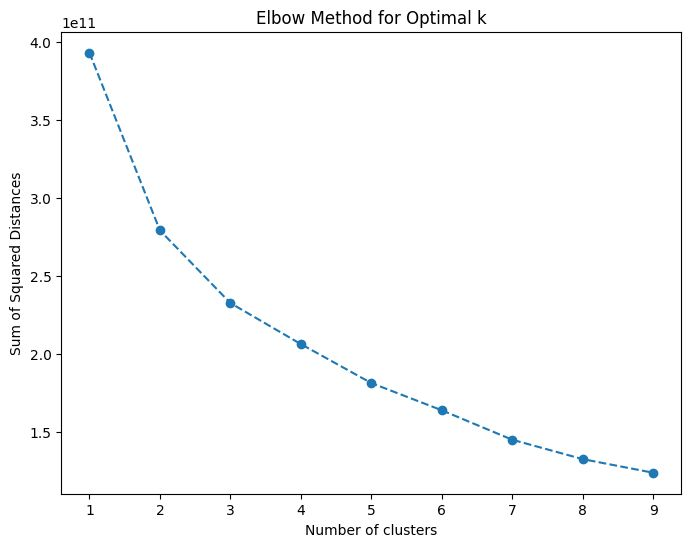
\includegraphics[width=0.4\linewidth]{elbow.jpeg} % Replace with your Elbow Curve image
    \caption{Elbow Method showing the optimal number of clusters for KMeans.}
    \label{fig:elbow_curve}
\end{figure}

After applying KMeans with \(k=4\), the clusters were visualized using t-SNE, as shown in Figure \ref{fig:kmeans_tsne}. The t-SNE plot shows distinct separations between clusters, indicating well-separated groups based on the feature set.

\begin{figure}[h]
    \centering
    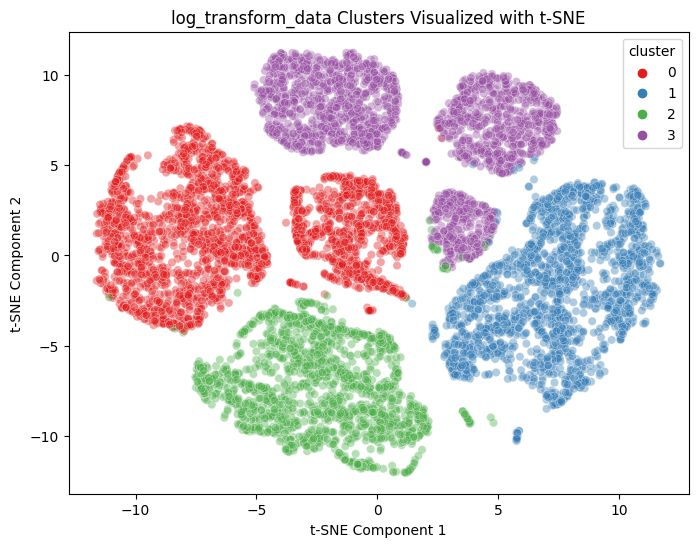
\includegraphics[width=0.4\linewidth]{kmeans-tsne.jpeg} % Replace with your KMeans t-SNE plot image
    \caption{t-SNE plot showing KMeans clusters.}
    \label{fig:kmeans_tsne}
\end{figure}

The KMeans algorithm was further evaluated using multiple metrics, including the Silhouette Score (0.4677), Calinski-Harabasz Index, and Davies-Bouldin Index, providing reasonable clustering results.

\subsection{Hierarchical Clustering}

Hierarchical clustering was applied to the dataset using various linkage methods. The dendrogram (Figure \ref{fig:dendrogram}) was used to determine the optimal number of clusters. Using the "complete" linkage method, four distinct clusters were identified.

\begin{figure}[h]
    \centering
    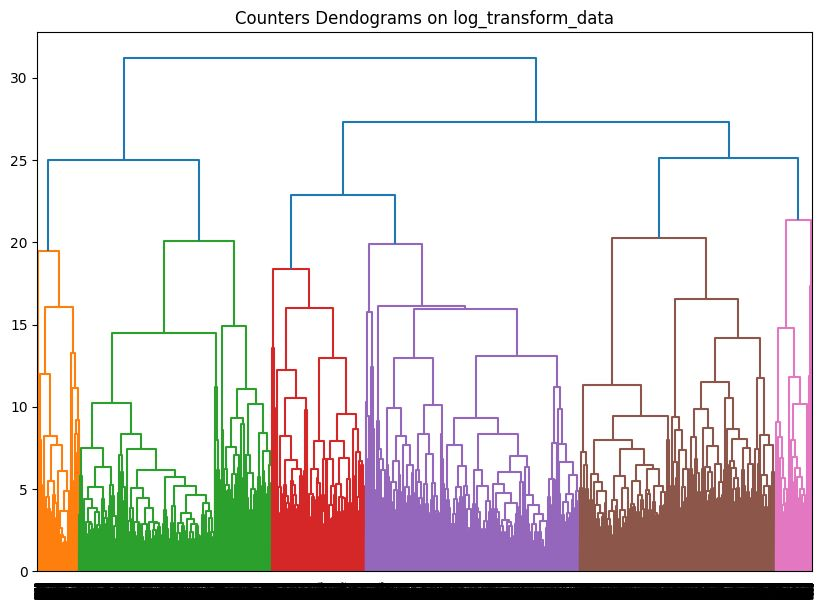
\includegraphics[width=0.4\linewidth]{dendogram.jpeg} % Replace with your Dendrogram image
    \caption{Dendrogram showing hierarchical clustering of the dataset.}
    \label{fig:dendrogram}
\end{figure}

The Silhouette Score for Hierarchical Clustering was 0.8543, which is higher than the score for KMeans, indicating that the hierarchical method produced better-defined clusters.

\subsection{DBSCAN Clustering}

DBSCAN was also tested on the dataset with various parameter settings. Using robust scaling, the clustering was visualized using t-SNE (see Figure \ref{fig:dbscan_tsne}).

\begin{figure}[h]
    \centering
    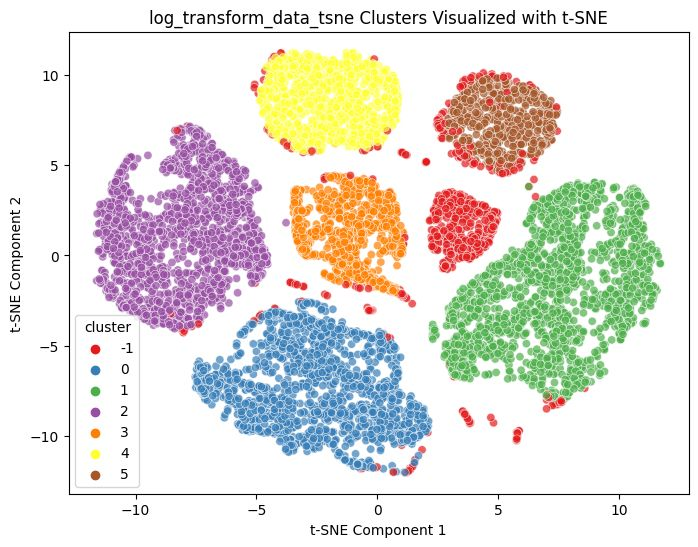
\includegraphics[width=0.4\linewidth]{dbscan-tsne.jpeg} % Replace with your DBSCAN t-SNE plot image
    \caption{t-SNE plot showing DBSCAN clusters.}
    \label{fig:dbscan_tsne}
\end{figure}

Despite some clusters being well-formed, the Silhouette Score for DBSCAN was lower (0.0812), indicating that the clusters were not as distinct.

\subsection{Gaussian Mixture Model (GMM)}

Finally, the Gaussian Mixture Model (GMM) was applied to the dataset. The t-SNE visualization of the clusters formed by GMM is shown in Figure \ref{fig:gmm_tsne}.

\begin{figure}[h]
    \centering
    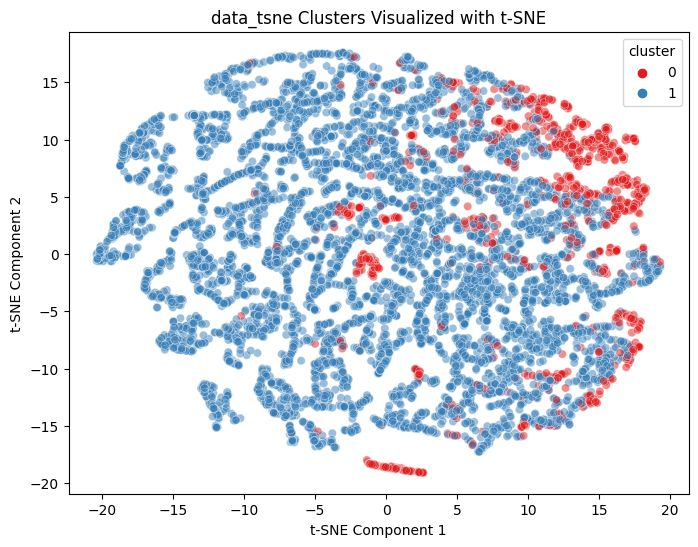
\includegraphics[width=0.4\linewidth]{gmm-tsne.jpeg} % Replace with your GMM t-SNE plot image
    \caption{t-SNE plot showing GMM clusters.}
    \label{fig:gmm_tsne}
\end{figure}

The Silhouette Score for GMM was 0.4579, which is comparable to KMeans but lower than Hierarchical Clustering.

As seen from the metrics, Hierarchical Clustering outperformed the other methods in terms of the Silhouette Score and overall cluster quality.

\subsection{Business Insights}

The clusters identified in the dataset provide valuable insights into customer behavior. These insights are critical for devising targeted marketing strategies and improving customer satisfaction.

\textbf{Cluster 0: High-Spenders with Frequent Large Purchases}

Customers in this cluster demonstrate very high balances and make frequent large purchases. They also have a high credit limit, indicating financial activity that may suggest they are high-value customers. Their purchasing behavior is primarily driven by large one-off transactions rather than smaller, routine payments. The high full-payment ratio suggests these customers manage their credit well, making them ideal for premium credit card offerings.

\textbf{Cluster 1: Installment-focused, Low One-off Activity}

This cluster consists of customers who prefer making installment purchases and avoid one-off transactions. They maintain high balances and make high minimum payments. They may benefit from installment-based financial products or services, such as loan options that allow them to spread payments over time. Financial institutions could offer tailored installment plans or discounts to cater to this group.

\textbf{Cluster 2: Moderate, Diverse Spenders}

These customers engage in both one-off and installment purchases but with more moderate activity than other clusters. They might represent a stable customer base with balanced financial behavior. Marketing campaigns could target this group with offers encouraging them to increase their use of credit, possibly through cashback or rewards programs for frequent transactions.

\textbf{Cluster 3: Cash Advance Heavy Users}

This group exhibits very high cash advance usage, significantly more than other clusters. The high balance and low full-payment ratio suggest liquidity issues or high short-term financial needs. Products such as short-term loans or overdraft facilities could be marketed to this cluster to address their immediate cash needs. Financial education programs may also help them better manage their credit to avoid large interest payments from frequent cash advances.

\section{Conclusion}

The aim of this study was to apply various clustering techniques to a dataset of credit card customers and evaluate their effectiveness in segmenting customers based on their behavioral patterns. We implemented \textit{KMeans}, \textit{Hierarchical Clustering}, \textit{DBSCAN}, and \textit{Gaussian Mixture Models (GMM)}, tuning the hyperparameters to find the optimal configuration for each method. Through our evaluation using metrics such as the \textit{Silhouette Score}, \textit{Calinski-Harabasz Index}, and \textit{Davies-Bouldin Index}, we identified the strengths and weaknesses of each algorithm.

Hierarchical Clustering and KMeans, particularly after PCA transformation, yielded the most promising results with well-defined clusters and strong performance metrics. \textit{Hierarchical Clustering} produced the best overall results with a \textit{Silhouette Score} of 0.8543, indicating that customers within each cluster were more homogeneous, and the separation between clusters was clearer. \textit{KMeans} with four clusters, as identified by the \textit{Elbow Method} and grid search, also performed well, providing insights into distinct customer groups with a moderate \textit{Silhouette Score} of 0.4677.

\textit{DBSCAN}, despite its ability to detect outliers, struggled with the dataset's structure and provided less meaningful clusters, evident from its low \textit{Silhouette Score}. On the other hand, \textit{Gaussian Mixture Models} performed moderately but were outclassed by KMeans and Hierarchical Clustering in this case, with a \textit{Silhouette Score} of 0.4579.

The clustering results yielded insightful business insights, which highlight different customer profiles. High spenders with frequent large purchases were identified, offering opportunities for premium services, while installment-focused customers represented a segment that could benefit from tailored installment plans. Moreover, cash advance-heavy users were identified as a high-risk group, suggesting a need for specialized financial products or credit counseling.

\section{Future Work}

In the future, more advanced clustering techniques, such as \textit{spectral clustering} or \textit{deep learning-based clustering}, could be explored to further enhance the segmentation. Additionally, incorporating external data such as demographic information or transaction histories may provide even richer insights. Finally, a deeper analysis of the clusters' stability and interpretability across different transformations could provide more robust solutions for customer segmentation.

\begin{thebibliography}{4}

\bibitem{jour} Xu, R., \& Tian, Y. (2015). A comprehensive survey of clustering algorithms. Annals of Data Science, 2(2), 165-193.

\bibitem{jour} Jain, A. K., \& Dubes, R. C. (2008). Algorithms for clustering data. Englewood Cliffs: Prentice Hall.

\bibitem{book} Tan, P.-N., Steinbach, M., \& Kumar, V. (2016). Introduction to data mining (2nd ed.). Boston: Pearson Addison-Wesley.

\bibitem{proceeding1} Ester, M., Kriegel, H. P., Sander, J., \& Xu, X. (1996). A density-based algorithm for discovering clusters in large spatial databases with noise. In Proceedings of the Second International Conference on Knowledge Discovery and Data Mining (pp. 226-231).

\bibitem{proceeding2} Ngai, E. W. T., Hu, Y., Wong, Y. H., Chen, Y., \& Sun, X. (2009). The application of data mining techniques in financial fraud detection: A classification framework and an academic review of literature. Decision Support Systems, 50(3), 559-569.

\bibitem{jour} Saraswat, A., \& Prakash, A. (2013). Segmentation of customers based on RFM analysis using K-Means clustering. International Journal of Computer Applications, 72(23), 37-40. 

\end{thebibliography}

\end{document}
